\chapter{Muistinhallinta} \label{Toinen luku}

Ohjelman muistin rakenteen ymmärtäminen on erityisen tärkeää tehokkaan muistin käytön saavuttamiseksi. Seuraavissa luvuissa tullaan esittelemään miten muistin allokointi ohjelmissa toimii
ja millaisista muistialueista ohjelman muisti koostuu. Huomioitavaa on, että seuraavaksi esiteltävä muistirakenne on tyypillisin muistirakenne, mistä tietokoneohjelman muisti koostuu. Ohjelman muistin rakenteeseen vaikuttaa mm. käytössä oleva suoritinarkkitehtuuri, ohjelmointikielen kääntäjä sekä kääntäjien tarjoamat muistin optimointityökalut.

\section{Ohjelman muisti}

Ohjelman muisti jakautuu erilaisiin muistialueisin. Koodiosa sisältää varsinaisesti ajettavan ohjelman binäärin eli ohjelmatiedoston, jonka prosessori suorittaa. Lisäksi ohjelmalla on olemassa dataosa, joka koostuu alustetusta datasta ja alustamattomasta datasta. Alustetun datan alueeseen kuuluvat globaalit ja staattiset muuttujat sekä vakioarvoiset muuttujat, joille on alustettu jokin arvo. Alustamattomassa data-alueessa on kaikki alustamaton data eli muuttujat, jotka ovat esitelty (declare), mutta joille ei ole annettu mitään arvoa. Näiden muistialueiden data allokoidaan ajettavan ohjelman muistiin jo käännön aikana (engl. \textit{compile time}) eli ohjelmointikielen kääntäjän kääntäessä lähdekoodin. Ohjelmalla on lisäksi myös kaksi muuta muistialuetta, pino ja keko. Tyypillisesti pino sijaitsee ylhäällä ja keko alhaalla ohjelman virtuaalisessa muistiavaruudessa.\cite{mmic2010} Pinon ja keon datan allokointi tapahtuu vasta ohjelman ajon aikana (engl. \textit{runtime}). Täsmennettävää on, että vaikka kääntäjän luomat ohjeet pinon hallintaan syntyvät jo käännön aikana, varsinainen datan allokointi ja vapautus tapahtuu ajon aikana. \cite{ddm2015book}

\begin{figure}[tbh]
{\begin{centering}
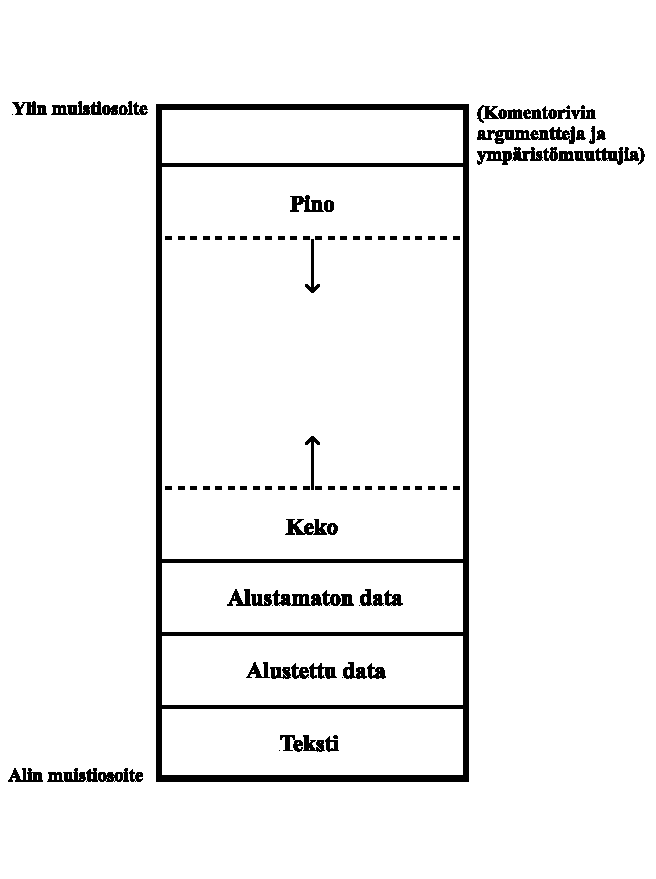
\includegraphics[width=0.6\textwidth]{kuvat/muistin_rakenne.pdf}
\par\end{centering}}
\caption{Ohjelman muistin rakenne \cite{mmic2010} (suomennettu kuva lähteestä)}
\end{figure}

/**Koodin pätkä**/

\subsection{Pino}

Pino (engl. \textit{stack}) on ohjelman muistialue, johon allokoidaan paikalliset muuttujat, funktioiden parametrit ja paluuosoitteet. Se noudattaa LIFO-periaateetta (engl. \textit{Last In First Out}) eli pinoon viimeiseksi puskettu data poistetaan pinosta myös ensimmäisenä. LIFO-periaatteen ansiosta pinoallokointi on tyypillisesti nopeampaa kuin kekoon allokoiminen, johtuen tavasta, miten pinon dataan päästään käsiksi. Lisäksi, pinon tavuja käytetään ohjelmassa säännöllisesti yhä uudelleen ja uudelleen, jolloin ne säilyvät hyvin prosessorin nopeassa välimuistissa. Data allokoidaan pinoon automaattisesti ja poistetaan sieltä, kun niiden näkyvyysalue päätyy. Pino koostuu kehyksistä (engl. \textit{frame}), joita pusketaan pinoon, kun ohjelma aloittaa uuden funktiokutsun suorittamisen. Tyypillisesti pinon koko on päätetty ennen ohjelman suorituksen aloittamista, ja pinoon allokoitavien muuttujien koko on tiedettävä etukäteen jo ennen kääntöä.\cite{mmic2010}
Pino-osoitin (engl. \textit{stack pointer}) pitää yllä tietoa muistiosoitteesta, jossa pinon viimeinen elementti sijaitsee. Tätä osoitinta muuttamalla, ohjelma pitää yllä tietoa mihin uusi kehys lisätään tai mistä vanha kehys poistetaan. Pino-osoitin pienenee, kun dataa pusketaan pinoon ja vastaisuudessa kasvaa, kun dataa poistetaan pinosta (huomioi pinon sijainti ohjelman muistiavaruudessa, kts. kuva 2.1).\cite{sasp2006}

\subsection{Keko}

Keko (engl. \textit{heap}, suom. myös \textit{heap}) on muistialue, johon kehittäjä allokoi sekä josta myös vapauttaa muuttujat manuaalisesti. Keko sisältää käytettävissä olevien ja vapaiden muistilohkojen linkitetyn listan. Keolle annetaan aloituskoko ohjelman suorituksen alkaessa, mutta muistinvaraaja voi pyytää sitä lisää tarvittaessa käyttöjärjestelmältä. Vastapainona pinolle, keko on hyödyllinen, kun ei voida tietää etukäteen kuinka paljon muistia tarvitsee varata ajon aikana.\cite{mmic2010} On syytä mainita, että tietokoneohjelman muistialue keko ei ole analogiassa tietorakenne keon kanssa.

\section{Muistin allokointi ohjelmointikielissä}

Muistia voidaan allokoida ohjelmalla kahdella tavalla, staattisesti tai dynaamisesti.

malloc, new

muistivuodot, segmentation fault

Dynaaminen muistinhallinta tuo kehittäjälle vapautta, mutta myös suuren vastuun. Edm. muistinkäytön ongelmatilanteet ja virheet voivat aiheuttaa päänvaivaa kokemattomalle kehittäjälle, mutta kokeneelle kehittäjälle osoittimet ja manuaalinen allokointi tarjoavat tehokkaat työkalut sovelluksen muistinkäytön tehostamiselle.

\begin{algorithm}[tbh]
\begin{minted}[fontsize=\small]{c}
#include <stdio.h>
#include <stdlib.h>

int i;  //Alustamaton muuttuja --> alustamaton data
int n = 1;  //Alustettu muuttuja --> alustettu data

int main(void)  //Funktiokutsu --> Pino
{  
    int numero = 10;    //Paikallinen muuttuja --> Pino
    int* osoitin = (int*)malloc(n * sizeof(int));   //Dynaamisesti allokoitu muistilohko --> Keko
    free(osoitin);  //Dynaamisesti vapautettu muistilohko --> Vapautettu keosta
    return 0;
}
\end{minted}
\caption{Demonstraatio muistin allokoinnista C-ohjelmointikielessä\label{alg:Demonstraatio}}
\end{algorithm}
